\label{testes}
\chapter{TESTES}

O presente capítulo tem como objetivo descrever quais foram os testes realizados durante o desenvolvimento do projeto Vocco a fim de garantir um controle de qualidade preciso da aplicação.

\section{Plano de testes}
 Nesta seção, será detalhado o modo como serão realizados os testes do sistema. Assim garantindo que as funções principais estejam de acordo com os requisitos propostos.

 \subsection{Teste de funcionalidade}
 
\begin{itemize}
    \item \textbf{Cenário Ideal Cadastro de Instituição:}
Descrição do cenário ideal de usabilidade do usuário no processo de cadastro de instituição.
    
\begin{figure}[ht]
        \centering
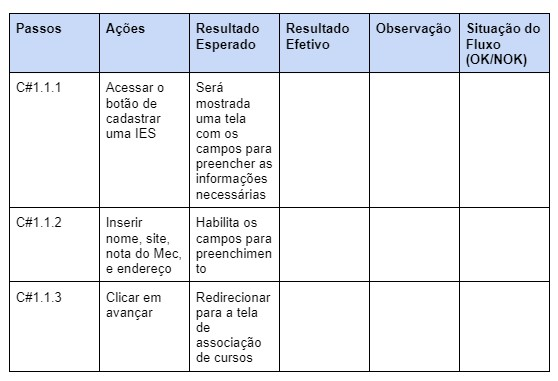
\includegraphics[width=0.80\textwidth]{images/teste-cad-instituicao-feliz.jpg}
        \caption{Cenário ideal cadastro de instituição}
        \label{commitsAturo}
    \end{figure}
O processo ideal de cadastro de instituição percorre três ações para ser concluído.

\newpage
    
    \item \textbf{Cenário de Exceção Cadastro de Instituição:}
Descrição do cenário de exceções de usabilidade do usuário no processo de cadastro de instituição.

\begin{figure}[ht]
        \centering
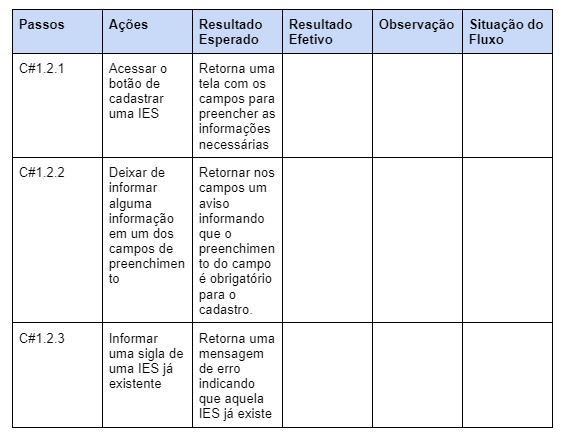
\includegraphics[width=0.80\textwidth]{images/teste-cad-instituicao-excecao.jpg}
        \caption{Cenário de exceção de cadastro de instituição}
        \label{commitsAturo}
    \end{figure}

O processo com exceções de cadastro de instituição percorre três ações para ser concluído.

\newpage
    
     \item \textbf{Cenário Ideal Listagem de Instituição:}
Descrição do cenário ideal de usabilidade do usuário no processo de listagem de instituição.

\begin{figure}[ht]
        \centering
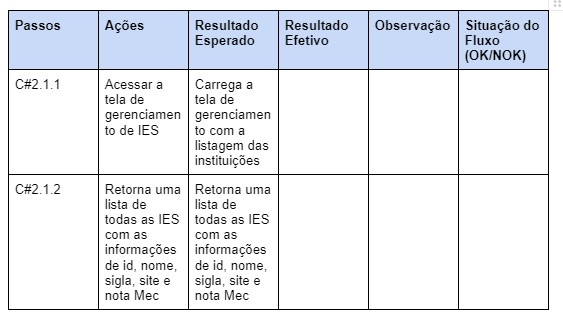
\includegraphics[width=0.80\textwidth]{images/teste-list-instituicao-feliz.jpg}
        \caption{Cenário ideal de Listagem de instituição}
        \label{commitsAturo}
    \end{figure}

O processo ideal de listagem de instituição percorre duas ações para ser concluído.


    \item \textbf{Cenário de Exceção Listagem de instituição:}
Descrição do cenário de exceções de usabilidade do usuário no processo de listagem de instituição.

\begin{figure}[ht]
        \centering
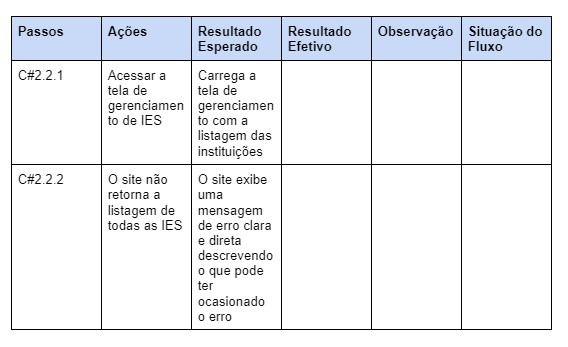
\includegraphics[width=0.80\textwidth]{images/teste-list-instituicao-excecao.jpg}
        \caption{Cenário de exceção de listagem de instituição}
        \label{commitsAturo}
    \end{figure}

O processo com exceções de listagem de instituição percorre duas ações para ser concluído.

\newpage
     
     \item \textbf{Cenário Ideal Detalhamento de instituição:}
Descrição do cenário ideal de usabilidade do usuário no processo de detalhamento de instituição.

\begin{figure}[ht]
        \centering
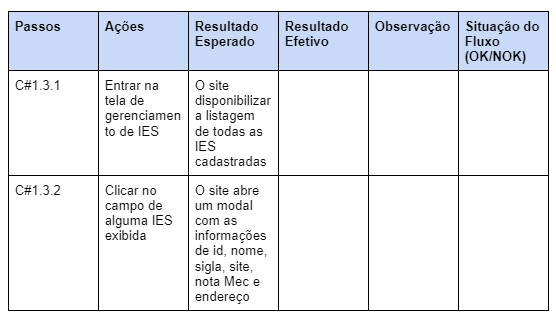
\includegraphics[width=0.80\textwidth]{images/teste-det-instituicao-feliz.jpg}
        \caption{Cenário ideal de detalhamento de instituição}
        \label{commitsAturo}
    \end{figure}

O processo ideal de detalhamento de instituição percorre duas ações para ser concluído.

\newpage

     \item \textbf{Cenário de Exceção Detalhamento de instituição:}
Descrição do cenário de exceções de usabilidade do usuário no processo de detalhamento de instituição.

\begin{figure}[ht]
        \centering
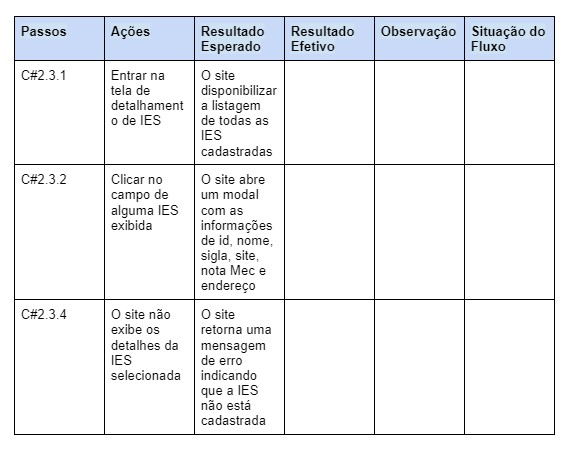
\includegraphics[width=1.0\textwidth]{images/teste-det-instituicao-excecao.jpg}
        \caption{Cenário de exceção de detalhamento de instituição}
        \label{commitsAturo}
    \end{figure}

O processo com exceções de detalhamento de instituição percorre três ações para ser concluído.

\newpage
     
     \item \textbf{Cenário Ideal Associação de Instituição com Curso:}
Descrição do cenário ideal de usabilidade do usuário no processo de associação de instituição com curso.

\begin{figure}[ht]
        \centering
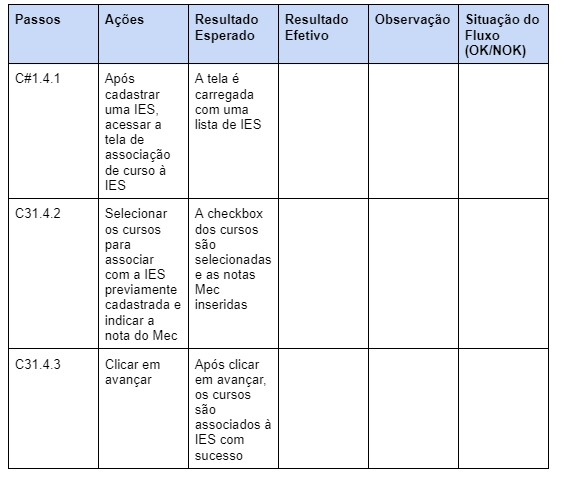
\includegraphics[width=1.0\textwidth]{images/teste-asso-instituicao-curso-feliz.jpg}
        \caption{Cenário ideal de associação de instituição com curso}
        \label{commitsAturo}
    \end{figure}

O processo ideal de associação de instituição com curso percorre três ações para ser concluído.


\newpage

\item \textbf{Cenário de Exceção Associação de Instituição com Curso:}
Descrição do cenário de exceções de usabilidade do usuário no processo de associação de instituição com curso.

\begin{figure}[ht]
        \centering
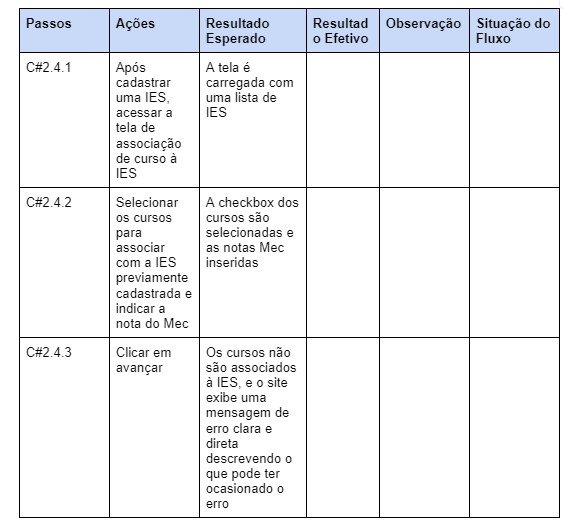
\includegraphics[width=1.0\textwidth]{images/teste-asso-instituicao-curso-excecao.jpg}
        \caption{Cenário de exceção associação de instituição com curso}
        \label{commitsAturo}
    \end{figure}

O processo com exceções de associação de instituição com curso percorre três ações para ser concluído.


\newpage

    \item \textbf{Cenário Ideal Exclusão de Instituição:}
Descrição do cenário ideal de usabilidade do usuário no processo de exclusão de instituição.


\begin{figure}[ht]
        \centering
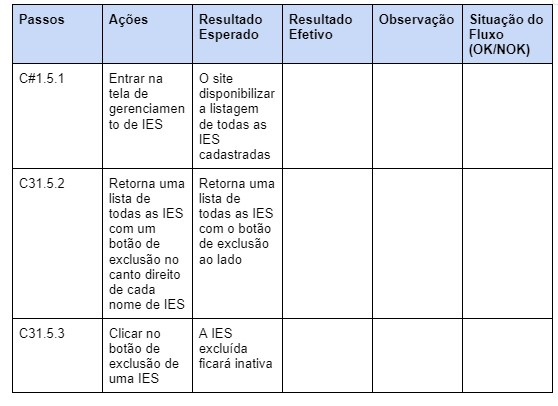
\includegraphics[width=1.0\textwidth]{images/teste-exc-instituicao-feliz.jpg}
        \caption{Cenário ideal de exclusão de instituição}
        \label{commitsAturo}
    \end{figure}

O processo ideal de exclusão de instituição percorre três ações para ser concluído.

\newpage

 \item \textbf{Cenário de Exceção Exclusão de Instituição:}
Descrição do cenário de exceções de usabilidade do usuário no processo de exclusão de instituição.

\begin{figure}[ht]
        \centering
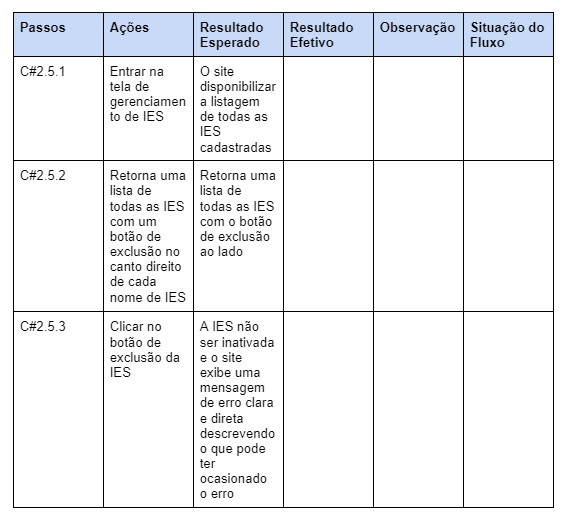
\includegraphics[width=0.75\textwidth]{images/teste-exc-instituicao-excecao.jpg}
        \caption{Cenário de exceção de exclusão de instituição}
        \label{commitsAturo}
\end{figure}
O processo com exceções de exclusão de instituição com curso percorre três ações para ser concluído.

\end{itemize}

A partir dos cenários de teste apresentados, torna-se viável simular um eventual caminho alternativo que o usuário final pode enfrentar durante a sua experiência navegando pelo site. Dessa forma, é possível realizar uma análise voltada à visão do usuário final, buscando suprir suas necessidades e melhorar a usabilidade do site.


\section{Teste de Usabilidade com Usuários}
Após o desenvolvimento da aplicação, foi realizado um teste de usabilidade com usuários previamente selecionados pela equipe com o objetivo de avaliar a interação e a funcionalidade do sistema. Para isso, foi disponibilizado o link da aplicação aos participantes, que foram orientados a explorar o maior número possível de funcionalidades oferecidas, como Cadastro, Login, Recuperação de Senha, Gestão de Conta, Teste Vocacional e Pesquisa de Cursos e Instituições. Após a utilização, os participantes preencheram um formulário de avaliação de usabilidade, que nos permitiu coletar dados qualitativos e quantitativos sobre a experiência de uso. A amostra foi composta por 20 participantes, cujas interações forneceram informações valiosas para a identificação de pontos fortes e áreas de melhoria, contribuindo para o aprimoramento contínuo do projeto.

O formulário de avaliação foi dividido em três blocos de perguntas:

\begin{itemize} 
\item Questionamento sobre o nível educacional atual do participante, categorizado entre estudante de ensino fundamental, ensino médio, ensino superior/pós-graduação ou não estudante. 
\end{itemize} 
\begin{itemize} 
\item Afirmações sobre a usabilidade da aplicação, que deveriam ser avaliadas de acordo com a experiência do usuário em uma escala de 1 a 5, sendo 1 "Discordo totalmente" e 5 "Concordo totalmente". 
\end{itemize} 
\begin{itemize} 
\item Perguntas para avaliar a utilidade percebida das três principais funcionalidades do sistema: Teste Vocacional, Listagem de Cursos e Listagem de Instituições. Além de um espaço aberto para sugestões de melhorias.  
\end{itemize}

Essas perguntas visaram fornecer uma compreensão da percepção dos usuários em relação à usabilidade, acessibilidade e utilidade das funcionalidades oferecidas pela aplicação, permitindo ajustes direcionados para otimizar a experiência do usuário.

\subsection{Resultados}
A seguir, será realizada a análise das respostas dos usuários no formulário disponibilizado. No apêndice \ref{apendice_l}, estão disponíveis todos os gráficos gerados no teste. Nesta seção, o foco está na análise dos resultados obtidos.

\subsection{Perfis dos participantes do teste}
A primeira pergunta do teste tinha como objetivo definir qual perfil o participante melhor se encaixa, entre as opções de estudante de ensino fundamental, ensino médio, superior / pós graduação ou não estudantes. Na figura \ref{fig:nivel} é possível verificar os resultados.

\newpage
\begin{figure}[ht]
        \centering
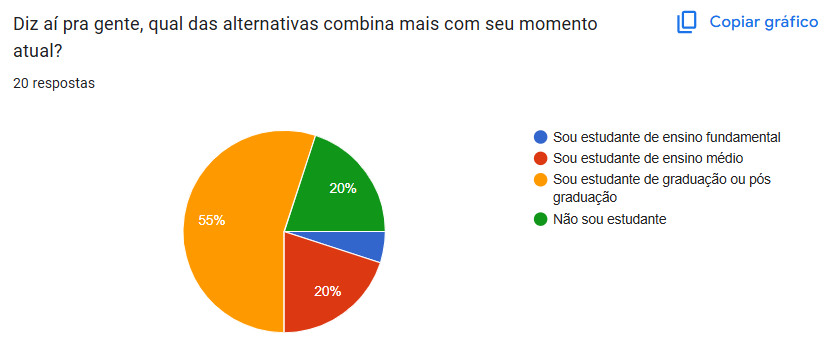
\includegraphics[width=1.0\textwidth]{images/estudante.png}
        \caption{Pergunta sobre nível de escolaridade do participante}
        \label{fig:nivel}
\end{figure}

Constatou-se que a maioria dos participantes do teste (55\%) são estudantes de graduação ou pós graduação, seguidos por estudantes de ensino médio (20\%), não estudantes (20\%) e estudantes de ensino fundamental(5\%). 

\subsection{Análise dos resultados}
As questões sobre a usabilidade do sistema presentes no formulário foram:

\begin{itemize} \item O sistema de cadastro e login carregou rapidamente e funcionou sem erros.
\item O processo de recuperação de senha foi fácil e concluído em pouco tempo.
\item O carregamento e a navegação na tela de teste vocacional foram rápidos e sem travamentos.
\item Os resultados do teste vocacional foram apresentados de forma clara e acessível.
\item O dashboard com resultados anteriores apresentou as informações de maneira organizada e carregou rapidamente.
\item A tela de instituições cadastradas possui filtros intuitivos e eficazes para busca.
\item A tela de cursos cadastrados apresenta informações relevantes, facilitando a localização do que é procurado.
\item O gerenciamento de conta foi intuitivo e atendeu às expectativas.
\item O processo para adicionar uma foto de perfil foi rápido e fácil.
\item Qual a relevância da sessão de Teste Vocacional?
\item Qual a relevância da sessão de Listagem de Instituições?
\item Qual a relevância da sessão de Listagem de Cursos?
\item No geral, minha experiência foi satisfatória.
\item Qual é sua opinião geral sobre a plataforma?
\item Você tem alguma sugestão para melhorar o desempenho ou a experiência do site?
\end{itemize}

Em relação às afirmações avaliativas, a maioria das respostas variou entre 4 (Concordo) e 5 (Concordo totalmente). A única exceção foi na questão sobre adicionar uma foto de perfil, em que um dos participantes enfrentou dificuldades para realizar o processo. O problema foi solucionado ao entrar em contato com o participante e auxiliá-lo, pois se tratava de um erro de escrita no email informado pelo usuário.

Sobre a relevância das sessões de Teste Vocacional, Listagem de Cursos e Listagem de Instituições, as respostas oscilaram entre 4 (Relevante) e 5 (Muito relevante).

Quanto à experiência geral do usuário e sua opinião sobre a plataforma, as respostas ficaram entre 4 (Satisfatória/Muito boa) e 5 (Muito satisfatória/Excelente).

Por fim, as sugestões de melhoria recebidas mostraram-se, em sua maioria, semelhantes ou repetitivas, destacando aspectos que não haviam sido identificados e que se revelaram importantes para os usuários. As sugestões mais recorrentes foram devidamente mapeadas e implementadas.

Os resultados estão alinhados com as expectativas do grupo, indicando que o público-alvo se identifica com a plataforma, aprecia as funcionalidades oferecidas e demonstra satisfação com seu desempenho e usabilidade.

\section{Teste de interface}
Foram realizados testes de interface \ac{e2e} utilizando a ferramenta Cypress para validar a funcionalidade da aplicação de forma completa. O Cypress nos permitiu simular interações do usuário com a interface, como navegação, preenchimento de formulários, e clique em botões, garantindo que todas as funcionalidades da aplicação estejam operando corretamente.

Durante o processo, foram desenvolvidos uma série de casos de teste que abrangem os fluxos principais da aplicação, garantindo que a interface funcione conforme esperado em diferentes cenários. As funcionalidades testadas incluem:

\begin{itemize}
    \item \textbf{Cadastro de usuários:} Verificou-se o fluxo completo de criação de contas, incluindo o preenchimento de dados, validação e confirmação.  
    \item \textbf{Login:} Avaliou-se o acesso à aplicação, garantindo autenticação e resposta ao inserir as credenciais.  
    \item \textbf{Seções do dashboard do estudante:} Validou-se o acesso às diferentes seções do dashboard, verificando o carregamento de informações e a funcionalidade da barra de pesquisa.  
    \item \textbf{Teste vocacional:} Foi testado o fluxo completo para a realização do teste vocacional, desde o início até a apresentação dos resultados.  
    \item \textbf{Deleção de conta:} Foi realizado o fluxo de deleção de conta.
\end{itemize}


\begin{figure}[ht]
        \centering
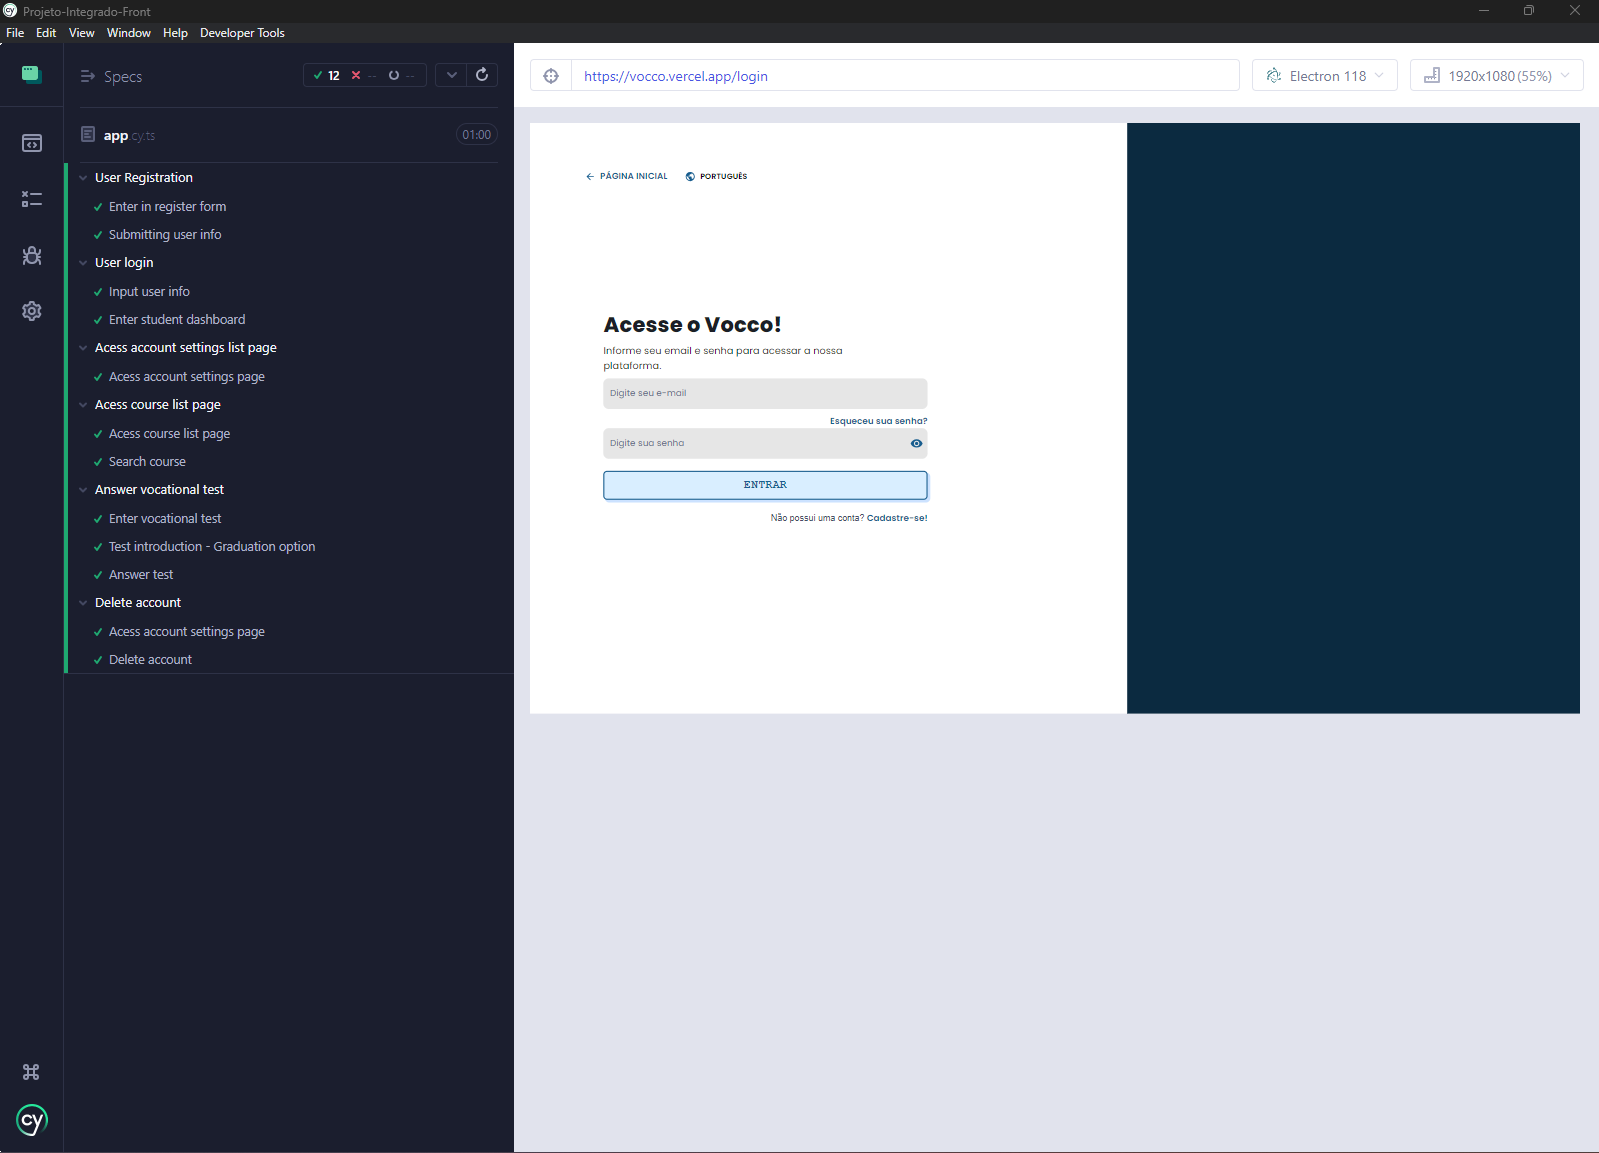
\includegraphics[width=1.0\textwidth]{images/e2e.png}
        \caption{Resultado do teste E2E com a ferramenta Cypress}
        \label{fig:e2e}
\end{figure}

Os testes foram executados de forma automatizada, como ilustrado na Figura \ref{fig:e2e}, proporcionando uma visão detalhada e em tempo real dos resultados obtidos. Além disso, é possível acompanhar a execução dos testes no canal do YouTube \textit{@AdasTechIFSP}, que apresenta um registro completo dos fluxos validados.  


\section{Testes de conformidade web}
Além dos testes anteriormente descritos, a aplicação também foi submetida a uma série de testes que avaliam aspectos técnicos e de conformidade com os padrões da \textit{web}. Nesse processo, realizou-se a validação do \ac{html}, a análise da configuração \ac{ssl} e a verificação das respostas \ac{http} emitidas pela aplicação, utilizando ferramentas especializadas.

Este capítulo detalha os métodos empregados para realizar essas validações, as ferramentas utilizadas para cada tipo de teste e como os resultados obtidos influenciam a qualidade e a segurança da aplicação.

\subsection{Validador de HTML}
A validação de \ac{html}  garante que o código-fonte segue os padrões estabelecidos pelo W3C, assegurando compatibilidade entre navegadores, acessibilidade para diferentes públicos e eficiência na renderização dos elementos visuais.

Para a validação do \ac{html}, foi utilizada a ferramenta Validator W3. Na Figura \ref{fig:html}, é possível observar que a ferramenta não apontou nenhum erro em relação ao \ac{html} da nossa aplicação, indicando que o código está devidamente estruturado e segue as boas práticas recomendadas.

\begin{figure}[ht]
        \centering
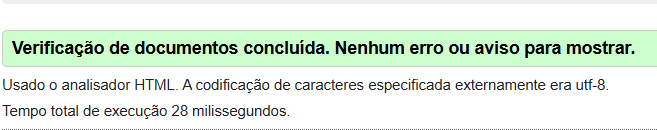
\includegraphics[width=1.0\textwidth]{images/html.png}
        \caption{Resultado da validação de html}
        \label{fig:html}
\end{figure}

Isso contribui para a compatibilidade entre navegadores e para a acessibilidade do sistema, aspectos essenciais para uma aplicação de qualidade.

\subsection{Teste de SSL}
O teste de \ac{ssl} é voltado para a análise da segurança das conexões criptografadas, verificando se o certificado digital está corretamente configurado e se a aplicação protege adequadamente os dados em trânsito, um requisito essencial para a confiança dos usuários.

Para validar a configuração e segurança do \ac{ssl}, utilizou-se a ferramenta Qualys SSL Labs, reconhecida pela sua capacidade de realizar uma análise confiável de certificados digitais e conexões seguras. Conforme ilustrado na Figura \ref{fig:ssl}, nossa aplicação alcançou a nota máxima (A+), indicando que as configurações do SSL atendem aos mais altos padrões de segurança, incluindo criptografia robusta, suporte a protocolos modernos e ausência de vulnerabilidades conhecidas.

\begin{figure}[ht]
        \centering
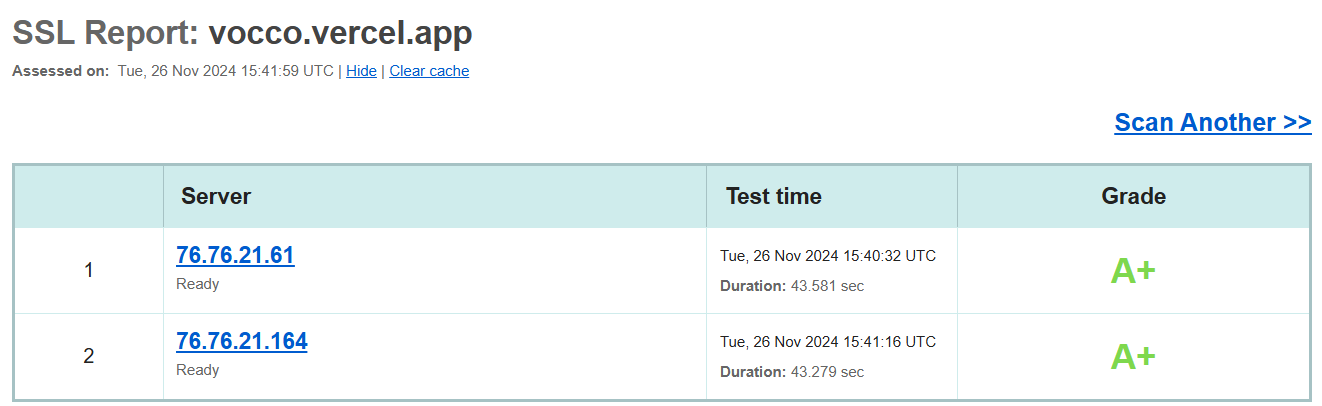
\includegraphics[width=1.0\textwidth]{images/ssl.png}
        \caption{Resultado da validação de ssl}
        \label{fig:ssl}
\end{figure}


Esse resultado reforça a confiabilidade e a robustez da aplicação no que diz respeito à proteção de dados sensíveis, garantindo uma experiência segura para os usuários.

\subsection{Teste de respostas HTTP}
A avaliação das respostas \ac{http} tem como objetivo verificar a adequação dos códigos de status, cabeçalhos e mensagens retornadas pelo servidor, contribuindo para o correto funcionamento de APIs e a entrega de uma experiência consistente ao usuário final.

Para validar as respostas \ac{http} da aplicação, foi utilizada a ferramenta Security Headers. Como apresentado na Figura \ref{fig:http}, a aplicação alcançou a nota máxima (A+), demonstrando conformidade com as melhores práticas, incluindo a implementação de políticas como Content-Security-Policy, Strict-Transport-Security e X-Frame-Options. Esse resultado destaca o compromisso com a proteção contra vulnerabilidades comuns e a segurança das interações entre usuários e o sistema.

\begin{figure}[ht]
        \centering
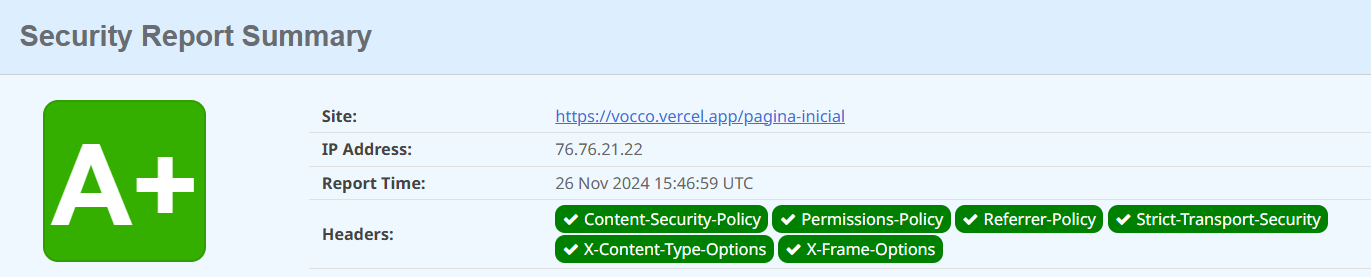
\includegraphics[width=1.0\textwidth]{images/http.png}
        \caption{Resultado da validação de respostas http}
        \label{fig:http}
\end{figure}


A obtenção dessa nota máxima evidencia que a aplicação está devidamente configurada para oferecer segurança e confiabilidade nas comunicações, alinhando-se aos padrões modernos de desenvolvimento web.


\chapter{CONSIDERAÇÕES FINAIS}

Este projeto teve como objetivo desenvolver uma plataforma que centraliza informações sobre educação técnica e de nível superior, disponibilizando detalhes sobre cursos e instituições, além de oferecer recomendações personalizadas de cursos com base em um teste vocacional fundamentado na teoria vocacional de John Holland. A proposta surgiu a partir da constatação, durante a revisão bibliográfica, da dificuldade enfrentada por estudantes de baixa renda ao escolherem uma profissão, muitas vezes devido à falta de orientação adequada e de acesso a informações centralizadas e confiáveis.

A plataforma foi construída com tecnologias modernas, seguras e confiáveis, garantindo uma experiência intuitiva e acessível para os usuários. O teste vocacional foi cuidadosamente implementado para identificar os perfis primário e secundário dos usuários, orientando-os de maneira assertiva em suas escolhas profissionais.

Após a realização de testes e a análise das respostas dos usuários, constatou-se que o público-alvo demonstrou alto grau de satisfação com a solução proposta. As funcionalidades da plataforma foram bem avaliadas, e as sugestões recebidas contribuíram para refinar ainda mais a aplicação. Esses resultados indicam que a ferramenta cumpre sua missão de ser uma aliada eficaz na orientação vocacional e no acesso à educação técnica e superior, sendo bem aceita pelos usuários.

Além disso, foram planejadas futuras implementações com o objetivo de ampliar e diversificar as informações disponíveis, tornando a plataforma mais completa. Melhorias serão feitas para facilitar a atualização de dados das instituições e cursos, além de possibilitar a interação entre os estudantes, promovendo o compartilhamento de experiências e o fortalecimento de uma comunidade voltada ao aprendizado e à troca de conhecimentos.

Com base nesses resultados e perspectivas, conclui-se que a plataforma atende às expectativas iniciais e possui grande potencial para impactar positivamente a vida dos estudantes, auxiliando-os em suas decisões profissionais de forma prática, acessível e eficiente, enquanto continua evoluindo para atender às suas necessidades futuras.
























